\part{Progettazione di un'interfaccia grafica per la compressione di immagini}

L'interfaccia grafica è realizzata con l'ambiente di sviluppo QT\cite{qt}, il quale permette di creare delle GUI scrivendo il codice in linguaggio c++. La compressione applicata è stata limitata ad un livello logico, ovvero l'immagine perde l'informazione legata alle alte frequenze, però le strutture dati che contengono tale immagine rimangono costanti. Introducendo però la possibilità ad un successivo salvataggio dell'immagine, nel quale vengono memorizzati solo i coefficienti diversi da 0.

Il programma fornisce una schermata nella quale è possibile selezionare l'immagine da comprimere e i valori di compressione da applicare. Nella sezione di sinistra viene mostrata l'immagine originale, mentre in quella di destra la sua versione compressa. In figura\ref{fig:deer} è riportato un esempio sull'immagine \textit{deer}, sulla quale sono stati applicati blocchi di elevate dimensioni (70x70) ed una bassa compressione (taglio ad 11 su 138 possibili), in questo modo è facilmente osservabile l'effetto della compressione.

Una feature fondamentale per la rapida compressione dell'immagine è stata l'aggiunta dei thread, in questo modo è stato possibile suddividere il lavoro e rendere la compressione quasi istantanea. La seguente implementazione è stata resa realizzata grazie all'indipendenza dei blocchi, tramite i quali è possibile allocare la memoria, eseguire la compressione e riscrivere i pixel in un nuovo oggetto immagine, in maniera parallela tra un blocco e l'altro.

\begin{figure}[h]
	\centering
	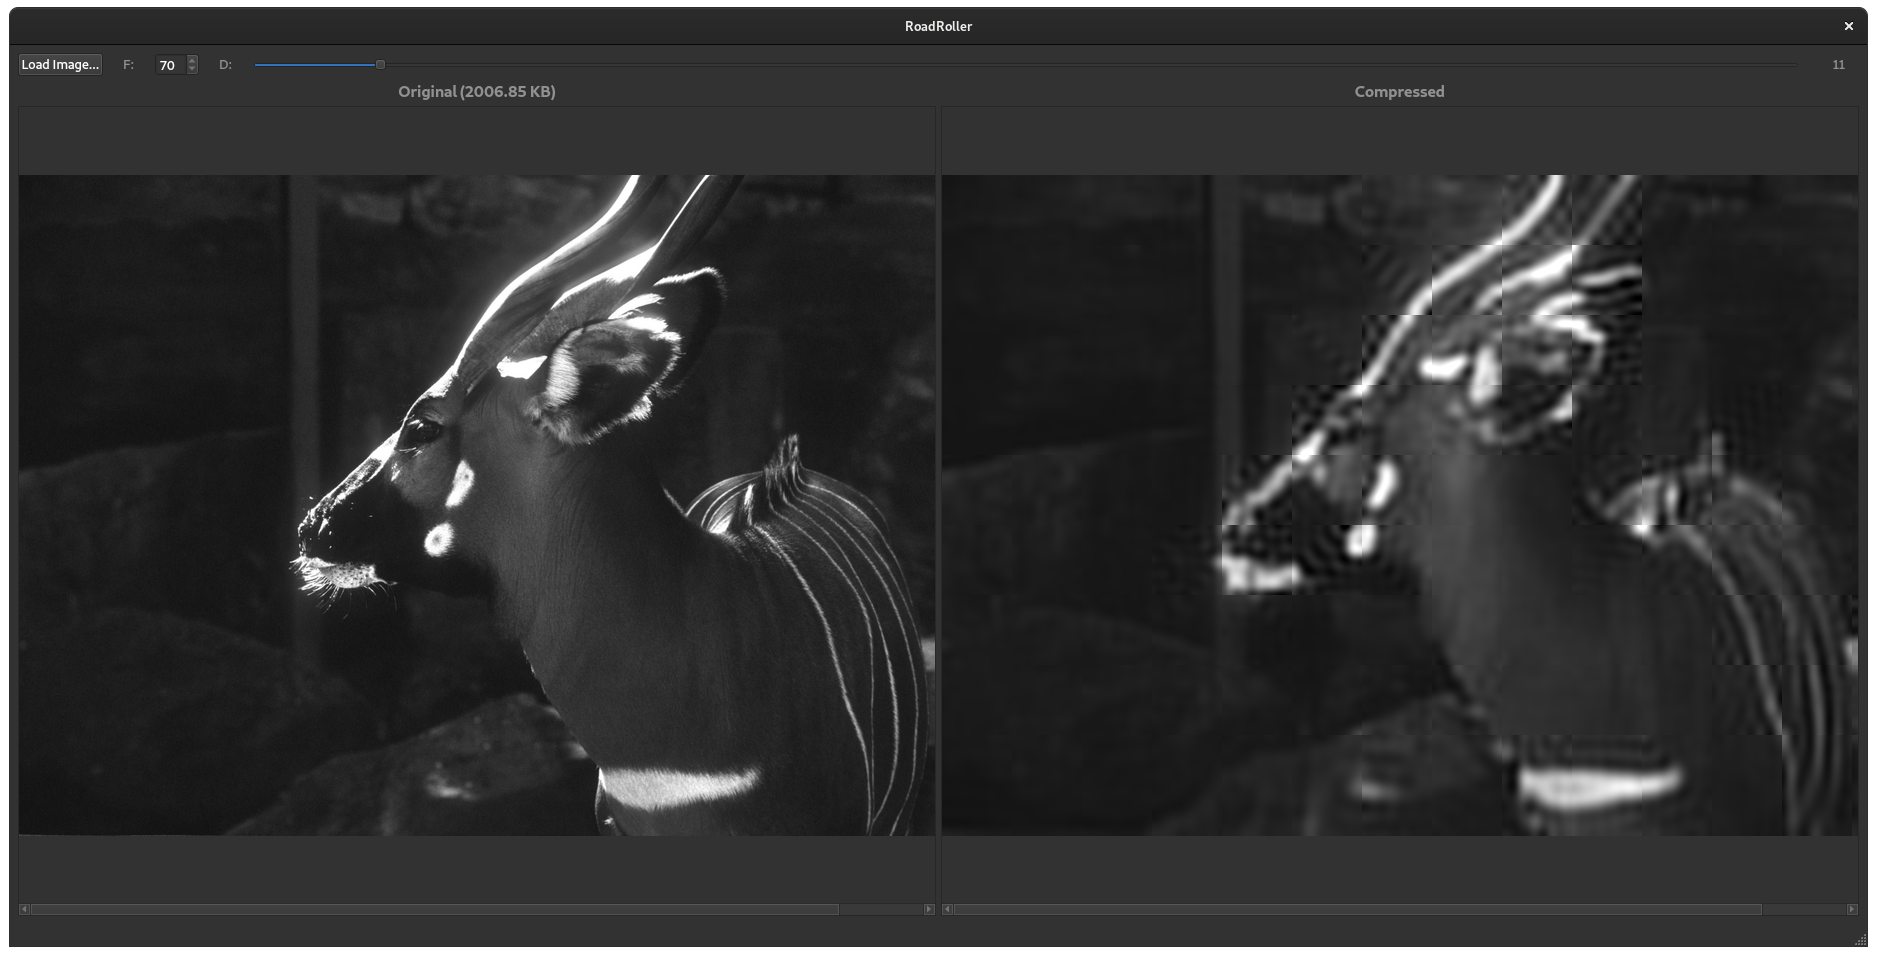
\includegraphics[width=1\linewidth]{figures/qt_deer}
	\caption{Programma di compressione con Qt}
	\label{fig:deer}
\end{figure}


Per osservare meglio la compressione potremmo momentaneamente saltare la conversione dei valori tramite la IDCT2. In figura\ref{fig:compression_values} viene mostrato il risultato ottenuto, dove è possibile osservare che la dct genera i valori dei coefficienti e successivamente questi vengono tagliati per il fattore fornito dall'interfaccia.

\begin{figure}[h]
	\centering
	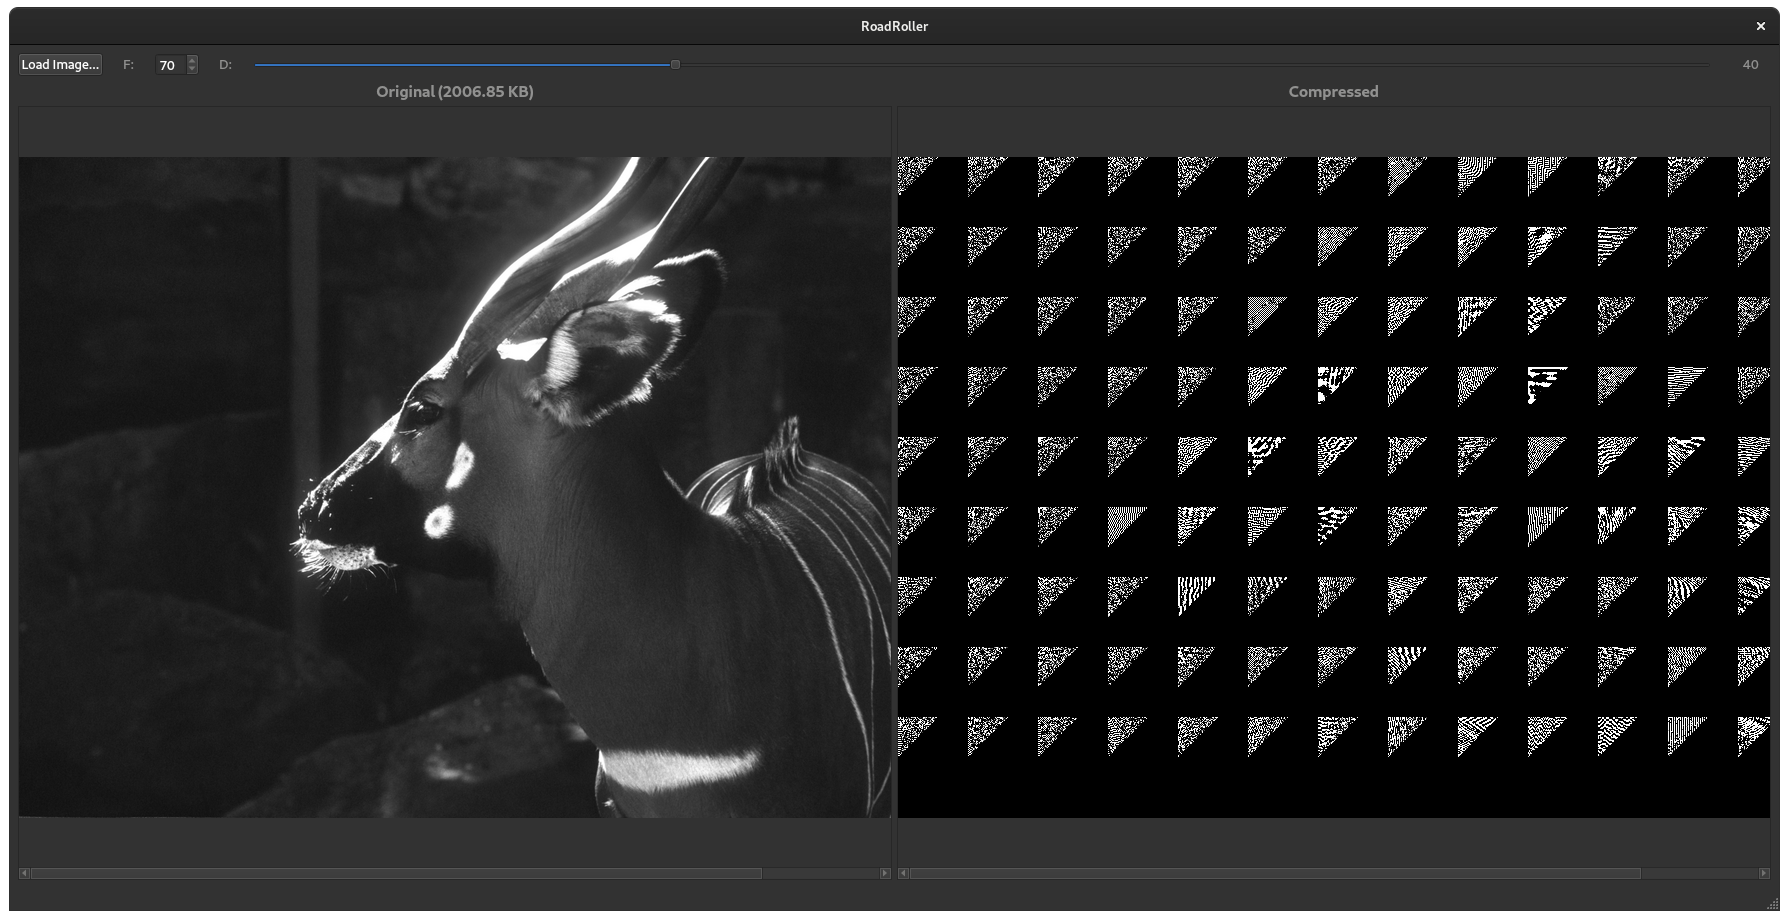
\includegraphics[width=1\linewidth]{figures/qt_dct_values}
	\caption{Valori della DCT generati dalla compressione}
	\label{fig:compression_values}
\end{figure}
